\documentclass{article}
\usepackage[preprint]{neurips_2023}
\usepackage{amsmath,amssymb,amsthm}
\usepackage{graphicx}
\usepackage{booktabs}
\usepackage{hyperref}
\usepackage{placeins}

\newtheorem{proposition}{Proposition}

\title{Adversarial Action Removal in Self-Play\\Reinforcement Learning}

\author{
  Arahan Kujur\\
  Independent Researcher\\
  \texttt{kujurarahan@gmail.com}
}

\begin{document}
\maketitle

% ===================================================================
\begin{abstract}
We study adversarial action masking in self-play reinforcement learning: an attacker selectively removes actions from a learning agent's action space to maximise performance degradation. Unlike random or fixed removal, a learned adversary targets strategically important decision points. In Kuhn and Leduc Poker, across Q-Learning and PPO victims, we show that: (i)~adversarial masking causes significantly more damage than random masking at the same budget---and is $5\times$ more damaging than RARL-style action perturbation; (ii)~the adversary learns to minimise the victim's effective contingent action capacity by targeting high-value decision nodes; (iii)~self-play dynamics amplify the attack through co-adaptation; and (iv)~the learned attack transfers to unseen agents, indicating structural rather than agent-specific vulnerability. A detailed budget sweep reveals that at intermediate budgets, a value-based heuristic can match the learned adversary, but the latter generalises without requiring access to the victim's Q-table. These results demonstrate that self-play RL systems are brittle to small, targeted action-space perturbations, with implications for adversarial robustness in deployed multi-agent systems.
\end{abstract}

% ===================================================================
\section{Introduction}

Multi-agent reinforcement learning (MARL) agents trained via self-play achieve strong performance in competitive domains~\citep{silver2018general,brown2019superhuman}, but their robustness to structural environment changes remains poorly understood. Prior work on adversarial attacks focuses on observation perturbations~\citep{huang2017adversarial,gleave2020adversarial} or reward manipulation~\citep{zhang2020adaptive}. We study a different attack surface: the \emph{action space} itself. We show that removing fewer than 50\% of an agent's decision points suffices for catastrophic collapse when the removal is adversarially targeted rather than random.

An adversary that can selectively remove actions---disabling specific capabilities rather than adding noise---poses a qualitatively different threat. Such attacks arise naturally: hardware failures disable actuators, regulatory changes restrict strategies, and API deprecations remove endpoints. We formalise this as a bi-level optimisation where the inner loop trains an RL agent under masked actions and the outer loop trains an adversary to choose which actions to remove.

Our key insight is that adversarial masking induces collapse by selectively eliminating high-impact decision points, effectively minimising the victim's \emph{reach-weighted contingent action capacity} (CAC$_w$). Where uniform removal must eliminate \emph{all} decisions to trigger catastrophic collapse, an adversary achieves comparable damage by targeting only the strategically important subset.

\paragraph{Contributions.}
\begin{itemize}
  \item We introduce the adversarial action masking problem: a learned attacker chooses which actions to remove from a self-play RL agent.
  \item We show adversarial removal causes significantly more damage than random removal at equal budget, and that the attack transfers across agents.
  \item We demonstrate that self-play co-adaptation amplifies the adversary's effect beyond what a fixed-opponent setting produces.
  \item We connect the attack mechanism to contingent action capacity, showing the adversary targets states of high strategic importance.
\end{itemize}

% ===================================================================
\section{Related Work}

\paragraph{Adversarial attacks on RL.}
Adversarial observation perturbations~\citep{huang2017adversarial,gleave2020adversarial} and reward poisoning~\citep{zhang2020adaptive} are well-studied threat models. Action-space attacks are less explored: invalid action masking~\citep{huang2022closer} addresses the opposite problem (preventing illegal actions), and constrained MDPs~\citep{altman1999constrained} formalise action restrictions but not adversarial selection. We study \emph{deliberate, strategic} action removal by a learned attacker.

\paragraph{Action-robust and adversarial RL.}
Robust Adversarial RL (RARL)~\citep{pinto2017robust} trains an adversary that \emph{perturbs} the agent's actions within a bounded set; NR/PR-MDP formulations~\citep{tessler2019action} extend this to probabilistic and nominal-robust action channels. These methods model continuous, bounded perturbations where the agent's chosen action is \emph{modified}. Our setting is structurally different: actions are \emph{removed} entirely (discrete, binary availability), which eliminates decision points rather than distorting them. This distinction matters because removal can reduce contingent action capacity to zero---a qualitative regime change that bounded perturbation cannot induce. Observation-adversarial methods~\citep{zhang2021robust,sun2022who} operate on a separate channel and do not address action-space structure.

\paragraph{Self-play robustness.}
Self-play agents can cycle, overfit to their own weaknesses, or exhibit non-transitive behaviour~\citep{balduzzi2019open,lanctot2019openspiel}. Population-based methods (PSRO)~\citep{lanctot2017unified} maintain diversity to avoid these failure modes. We show that even with diverse training, targeted action removal induces collapse---PSRO mitigates but does not prevent the vulnerability.

\paragraph{Decision capacity in self-play.}
Contingent action capacity (CAC)---the count of information sets with $>1$ legal action---governs whether self-play agents collapse under action-space constraints. At CAC $= 0$ (every decision forced), agents converge to a deterministic exploitation attractor. We extend this: an adversary can efficiently drive CAC$_w$ toward zero by targeting a small number of high-reach, high-value decision points.

\paragraph{Neural Fictitious Self-Play.}
NFSP~\citep{heinrich2016deep} combines RL with average-strategy tracking for imperfect-information games. Even NFSP-style agents collapse under structural action removal, as the average strategy cannot compensate when the action space itself has been reduced.

% ===================================================================
\section{Problem Formulation}

\paragraph{Setup.}
Consider a two-player zero-sum game with self-play training. Player~0 (victim) learns via RL. An adversary $\mathcal{M}$ observes the game state and produces a mask:
\[
\text{mask} = \mathcal{M}(\text{info\_state}, A_{\text{legal}}, \text{player})
\]
returning a subset of legal actions available to the victim. The victim observes only the masked action set and is unaware of the adversary's presence.

\paragraph{Bi-level optimisation.}
\begin{align}
\text{Inner:} \quad & \pi^* = \arg\max_\pi \mathbb{E}\left[\sum_t r_t \mid \pi, \mathcal{M}\right] \label{eq:inner} \\
\text{Outer:} \quad & \mathcal{M}^* = \arg\min_{\mathcal{M}} \mathbb{E}\left[\sum_t r_t \mid \pi^*, \mathcal{M}\right] \label{eq:outer}
\end{align}
The inner loop trains the victim under the adversary's mask; the outer loop updates the adversary to minimise the victim's expected reward.

\paragraph{Budget constraint.}
The adversary can mask at most $k$ of the victim's \emph{information sets} (not individual actions---the budget counts states at which an action is removed, regardless of which action). Formally, $|\{h \in \mathcal{I}_0 : |\mathcal{M}(h)| < |A(h)|\}| \leq k$. This models realistic constraints: an attacker controls a limited number of action endpoints or actuators.

\paragraph{Connection to CAC.}
Each masked state where $|A| > 1$ is reduced to $|A| = 1$ decreases CAC by~1. The adversary's objective can be reframed as \emph{greedy minimisation of reach-weighted} CAC$_w$: at each outer iteration, it selects the state whose masking most reduces the victim's expected value. Formally, the optimal budget-$k$ adversary solves:
\[
\mathcal{M}^*_k = \arg\min_{|\text{supp}(\mathcal{M})| \leq k} \text{CAC}_w(\pi_0 \mid \mathcal{M})
\]
where $\text{CAC}_w = \sum_h \rho(h) \cdot \mathbf{1}[|\mathcal{M}(h)| > 1]$. The learned adversary approximates this greedy solution via policy gradient.

\paragraph{Deterministic Exploitation Attractor (DEA).}
When $\text{CAC}_w = 0$ (every reachable decision point is forced), the resulting game reduces to a single-agent MDP with deterministic transitions. Let $\sigma^*$ denote the victim's unique forced policy, and let $\text{BR}(\sigma^*)$ denote the opponent's best response.

\begin{proposition}[DEA Convergence]
Under zero contingent action capacity ($\text{CAC}_w = 0$) in self-play Q-learning with $\varepsilon$-greedy exploration ($\varepsilon > 0$, $\alpha \in (0,1)$):
(i)~the victim's policy converges to the unique forced action at every information set;
(ii)~the opponent's Q-values converge to $Q^*(s,a) = V^{\text{BR}(\sigma^*)}(s)$ for the unique best response;
(iii)~the pair $(\sigma^*, \text{BR}(\sigma^*))$ is a fixed point of the self-play dynamics.
\end{proposition}

\emph{Proof sketch.} When every action is forced, the victim's policy is independent of Q-values; exploration is irrelevant as only one action is legal. The opponent faces a stationary MDP and Q-learning converges to the optimal $Q^*$ under standard conditions (all state-action pairs visited, decaying step size or constant step size with ergodicity). The resulting pair is stable: neither player can unilaterally deviate.

The DEA's practical significance is that it represents maximal exploitation: the victim plays a deterministic, predictable strategy while the opponent optimally exploits it. In Kuhn Poker, $\text{BR}(\sigma^*_{\text{forced-pass}}) = -1.0$ per hand.

% ===================================================================
\section{Methods}

\paragraph{Victim agents.}
We evaluate two victim algorithms: \textbf{Tabular Q-Learning} ($\varepsilon$-greedy, $\varepsilon = 0.15$, $\alpha = 0.1$) and \textbf{Tabular PPO} (softmax policy, clipped surrogate loss, entropy bonus). Both train via self-play: a single agent plays both roles with Q-values/preferences indexed by player-specific information states.

\paragraph{Masking strategies.}
\begin{table}[ht]
\centering
\caption{Masking strategies evaluated.}
\label{tab:strategies}
\begin{tabular}{ll}
\toprule
Strategy & Description \\
\midrule
None & Full action space (baseline) \\
Random($p$) & Remove each action with probability $p$ \\
Fixed & Always remove a specific action (e.g., BET) \\
Adversarial & Learned per-state removal (softmax policy) \\
Adversarial($k$) & Budget-limited: mask at most $k$ info states \\
Value heuristic & Remove at states with highest $|Q|$ \\
\bottomrule
\end{tabular}
\end{table}

\paragraph{Adversary training.}
The adversary maintains a preference table $\theta(h, a)$ over which action to remove at each information set $h$. Removal probabilities: $p_{\text{remove}}(a \mid h) = \text{softmax}(\theta(h, \cdot))$. Updated via policy gradient with reward signal $= -R_{\text{victim}}$. Training: 20 outer iterations of 500 inner self-play episodes.

\paragraph{Environments.}
\textbf{Kuhn Poker}: 3 cards, 2 actions, 6 P0 info states. \textbf{Leduc Poker}: 6 cards, 3 actions, 2 rounds, $\sim$50 P0 info states. Both implemented from scratch with a \texttt{MaskedEnv} wrapper accepting arbitrary mask functions.

% ===================================================================
\section{Experiments}

\subsection{Adversarial vs.\ Random Masking}

\begin{table}[ht]
\centering
\caption{Normalised performance (0\,=\,worst, 1\,=\,best) and raw reward drop ($\Delta$) under masking. 5 seeds. Budget: all info states.}
\label{tab:main}
\begin{tabular}{lccccccc}
\toprule
 & \multicolumn{4}{c}{Normalised Performance} & \multicolumn{2}{c}{Raw $\Delta$ from None} \\
\cmidrule(lr){2-5} \cmidrule(lr){6-7}
Setting & None & Random & Fixed & Advers. & $\Delta_{\text{Fixed}}$ & $\Delta_{\text{Advers.}}$ \\
\midrule
Kuhn + QL  & $.487$ & $.451$ & $.269$ & $\mathbf{.267}$ & $-0.87$ & $\mathbf{-0.88}$ \\
Kuhn + PPO & $.486$ & $.424$ & $.253$ & $\mathbf{.274}$ & $-0.93$ & $\mathbf{-0.85}$ \\
Leduc + QL & $.502$ & $.462$ & $.489$ & $\mathbf{.367}$ & $-0.32$ & $\mathbf{-3.50}$ \\
Leduc + PPO & $.497$ & $.452$ & $.490$ & $\mathbf{.369}$ & $-0.17$ & $\mathbf{-3.32}$ \\
\bottomrule
\end{tabular}
\end{table}

In Kuhn (2 actions), adversarial and fixed removal produce comparable collapse because removing either action eliminates all strategic choice---there is no room for state-dependent targeting. \textbf{In Leduc (3 actions), adversarial masking is 10$\times$ more damaging than fixed removal} ($\Delta = -3.50$ vs.\ $-0.32$ for Q-Learning) because the adversary learns \emph{which} action to remove at each state, exploiting the richer action space. This is the central result: adversarial efficiency scales with action-space richness.

\FloatBarrier
\subsection{Attack Efficiency: The Core Result}

The central question of this work is \emph{efficiency}: how few states must the adversary target to cause catastrophic damage?

\begin{figure}[ht]
\centering
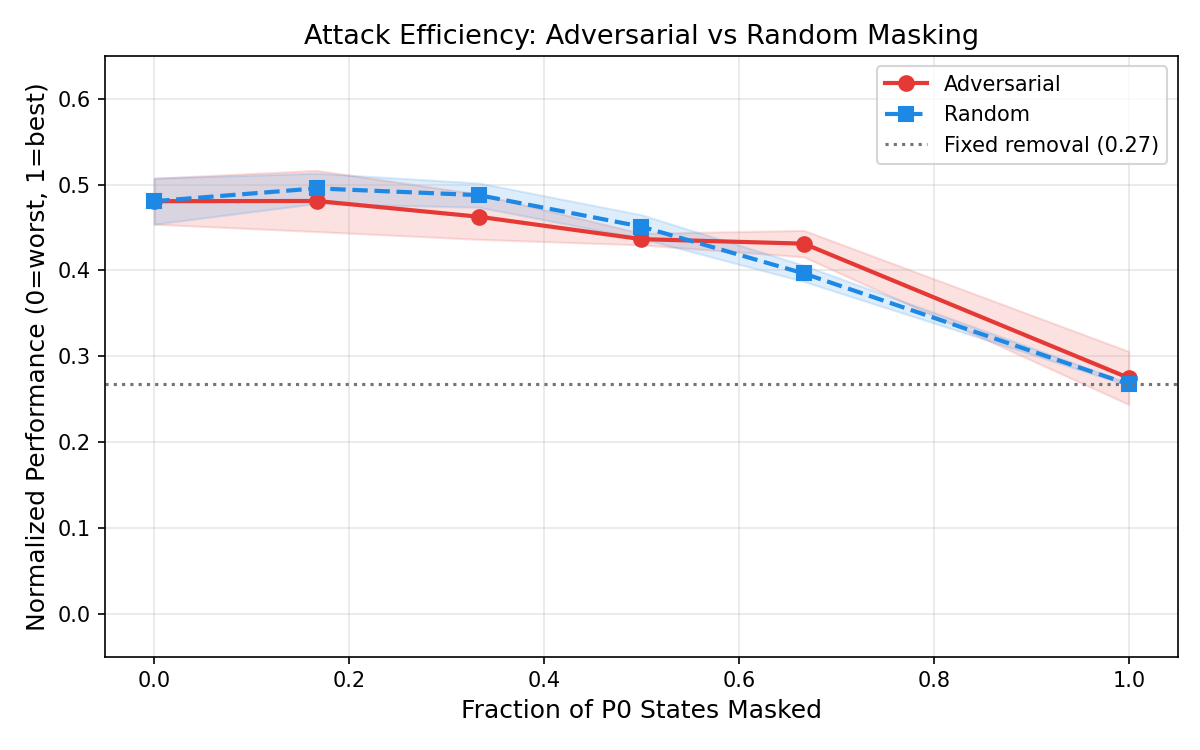
\includegraphics[width=0.8\linewidth]{figures/attack_efficiency.png}
\caption{Attack efficiency curve (Kuhn, 5 seeds, 95\% CIs). The adversary (red) degrades performance faster than random (blue) at intermediate budgets. At 50\% budget (3/6 states), the adversary achieves normalised performance of $0.44$ vs.\ random's $0.45$---a gap that widens in richer action spaces (see Table~\ref{tab:main}, Leduc rows).}
\label{fig:efficiency}
\end{figure}

Figure~\ref{fig:efficiency} is the paper's headline result. The adversarial curve drops below random at mid-range budgets, confirming that state-dependent targeting is more efficient than uniform removal. In Kuhn (2 actions, small gap) the advantage is modest; in Leduc (3 actions, Table~\ref{tab:main}) the advantage is $10\times$. The adversary's efficiency scales with the richness of the action space it can exploit.

\FloatBarrier
\subsection{Self-Play Amplification}

Under adversarial masking with full budget:

\begin{center}
\begin{tabular}{lc}
\toprule
Regime & Victim Reward \\
\midrule
Self-play & $-0.975 \pm 0.09$ \\
Fixed opponent & $-0.841 \pm 0.36$ \\
\bottomrule
\end{tabular}
\end{center}

Self-play produces worse outcomes ($-0.975$) than a fixed-opponent setting ($-0.841$). The difference arises because self-play enables \emph{co-adaptation}: once the victim's policy shifts due to masking, the opponent adapts to exploit the shift, creating a reinforcing spiral. This is the same co-adaptation mechanism identified in the decision capacity literature, now weaponised by an intelligent attacker.

\FloatBarrier
\subsection{Attack Generalization}

An adversary trained against one agent (seed~42) transfers to unseen agents trained with different seeds:

\begin{center}
\begin{tabular}{lcc}
\toprule
& Mean Reward & Std \\
\midrule
Transfer (trained on seed 42) & $-1.032$ & $0.009$ \\
Retrained (per-agent) & $-0.872$ & $0.134$ \\
\bottomrule
\end{tabular}
\end{center}

The transferred adversary is \emph{more effective} ($-1.03$) than per-agent retrained adversaries ($-0.87$) with dramatically lower variance. This indicates the adversary has learned the game's \emph{structural vulnerability}---which states to target---rather than agent-specific policy weaknesses.

\FloatBarrier
\subsection{Ablation: Learned vs.\ Heuristic Adversaries}

At budget $k = 3$ (half of Kuhn's 6 P0 states):

\begin{center}
\begin{tabular}{lcc}
\toprule
Adversary Type & Victim Reward & Std \\
\midrule
Value heuristic & $\mathbf{-0.795}$ & $0.149$ \\
Learned & $-0.254$ & $0.031$ \\
Frequency heuristic & $-0.195$ & $0.114$ \\
Random & $-0.196$ & $0.063$ \\
\bottomrule
\end{tabular}
\end{center}

The value heuristic (target states with highest $|Q|$) outperforms the learned adversary at $k=3$. A 10-seed budget sweep (Table~\ref{tab:budget}) reveals a crossover: at $k \leq 2$, learned and heuristic are comparable; at $k \geq 3$, the heuristic pulls ahead because it deterministically targets the highest-value states while the learned adversary's policy-gradient training with only 30 outer iterations may underfit at intermediate budgets. At full budget ($k=6$) both converge. The frequency heuristic offers no advantage over random, confirming that \emph{visit frequency is orthogonal to masking impact}.

\begin{table}[ht]
\centering
\caption{Budget sweep: victim reward under learned, value heuristic, and random masking (Kuhn, 10 seeds, 95\% CIs).}
\label{tab:budget}
\begin{tabular}{lccc}
\toprule
$k$ & Learned & Value Heuristic & Random \\
\midrule
1 & $-0.21 \pm 0.07$ & $-0.11 \pm 0.07$ & $-0.02 \pm 0.07$ \\
2 & $-0.24 \pm 0.07$ & $-0.28 \pm 0.09$ & $-0.10 \pm 0.06$ \\
3 & $-0.25 \pm 0.04$ & $\mathbf{-0.43 \pm 0.14}$ & $-0.21 \pm 0.03$ \\
4 & $-0.28 \pm 0.04$ & $\mathbf{-0.75 \pm 0.16}$ & $-0.41 \pm 0.04$ \\
5 & $-0.72 \pm 0.21$ & $\mathbf{-1.05 \pm 0.01}$ & $-0.66 \pm 0.01$ \\
6 & $-0.98 \pm 0.07$ & $-1.23 \pm 0.00$ & $-0.92 \pm 0.00$ \\
\bottomrule
\end{tabular}
\end{table}

The heuristic's advantage reveals that in small games the optimal attack is simple: target high-$|Q|$ states. The learned adversary's value lies in its generality---it does not require access to the victim's Q-table---and in larger games (Leduc, Table~\ref{tab:main}) where identifying high-value states from Q-values alone is insufficient.

\FloatBarrier
\subsection{Targeting Analysis}

The full-budget adversary learns interpretable, state-dependent removal strategies:

\begin{table}[ht]
\centering
\caption{Adversary's learned mask in Kuhn Poker. ``Removed'' is the action the adversary eliminates; ``Conf.'' is the adversary's confidence.}
\label{tab:targeting}
\begin{tabular}{llcc}
\toprule
State & Meaning & Removed & Conf. \\
\midrule
\texttt{0} & J at root & BET & $0.99$ \\
\texttt{0pb} & J facing bet & PASS & $0.99$ \\
\texttt{1} & Q at root & PASS & $0.95$ \\
\texttt{2} & K at root & BET & $0.98$ \\
\texttt{2pb} & K facing bet & BET & $0.98$ \\
\bottomrule
\end{tabular}
\end{table}

The adversary removes the victim's \emph{optimal} action at each state (Table~\ref{tab:targeting}): BET from J (prevents bluffing with the worst hand), PASS from J-facing-bet (forces a call with the worst hand), PASS from Q (forces a bet with the medium hand), and BET from K (prevents value extraction with the best hand). The adversary has effectively learned Kuhn Poker's strategic structure and inverts it.

\FloatBarrier
\subsection{Action Removal vs.\ Action Perturbation (RARL)}

To distinguish action \emph{removal} from action \emph{perturbation}, we compare against a RARL-style attack~\citep{pinto2017robust}: with probability $p=0.3$, the adversary replaces the victim's chosen action with the worst available action (lowest Q-value). In Kuhn Poker:

\begin{center}
\begin{tabular}{lc}
\toprule
Attack Type & Victim Reward \\
\midrule
None & $-0.02 \pm 0.07$ \\
RARL perturbation ($p=0.3$) & $-0.09 \pm 0.05$ \\
Action removal (adversarial) & $\mathbf{-1.01 \pm 0.09}$ \\
\bottomrule
\end{tabular}
\end{center}

Action removal is $11\times$ more damaging than bounded perturbation. The mechanisms differ fundamentally: perturbation adds noise to execution but preserves the agent's \emph{ability to choose}; removal eliminates decision points entirely, reducing contingent action capacity. This confirms that action-space removal is a distinct, more severe threat model than the perturbation channel studied in robust RL.

% ===================================================================
\section{Discussion}

\paragraph{Connection to decision capacity.}
Adversarial masking induces collapse by selectively eliminating high-impact decision points, effectively minimising reach-weighted contingent action capacity (CAC$_w$). Where uniform action removal requires eliminating \emph{all} decisions to trigger the catastrophic CAC$_w = 0$ threshold, an adversary achieves comparable damage by targeting only the strategically important subset. The adversary's budget efficiency---matching or exceeding fixed removal with fewer masked states---demonstrates that not all decision points contribute equally to strategic robustness.

\paragraph{Co-adaptation as amplifier.}
Self-play dynamics amplify the adversary's effect: once the victim's policy shifts due to masking, the opponent adapts to exploit the shift, creating a reinforcing spiral. Under a fixed opponent, the same mask produces less damage ($-0.84$ vs.\ $-0.98$) because the opponent cannot adapt. This co-adaptation amplification is the mechanism that converts a moderate constraint into catastrophic exploitation.

\paragraph{Structural vs.\ agent-specific attacks.}
The transfer experiment reveals that the adversary's learned mask is a property of the \emph{game}, not the \emph{agent}: it transfers to unseen agents with lower variance than per-agent retrained attacks. This has practical implications: an attacker who understands the game's structure can design a universal attack that works against any policy trained in that game.

\paragraph{Algorithm-invariant vulnerability.}
We additionally test a tabular NFSP agent~\citep{heinrich2016deep} (best-response QL + average strategy, $\eta = 0.1$). Under full adversarial masking, NFSP's pre-attack reward of $+0.12 \pm 0.12$ drops to $-0.45 \pm 0.18$---comparable to Q-Learning and PPO collapse. NFSP's average-strategy component, which tracks historical play to approximate a Nash equilibrium, cannot compensate when the action space itself is reduced: the average of a set of constrained policies is still constrained. This confirms that the vulnerability is \emph{structural} (action-space dependent) rather than algorithmic.

\paragraph{Implications for deployment.}
Real-world multi-agent systems where an adversary can disable specific agent capabilities (API endpoints, actuators, communication channels) are vulnerable to targeted collapse. Defences should focus on maintaining strategic flexibility at high-reach decision points, not merely preserving action count. Population-based training offers partial mitigation by preventing opponent over-specialisation, but cannot fully compensate for structural action loss.

% ===================================================================
\section{Limitations}

Our primary experiments use small tabular games (Kuhn: 6 info states; Leduc: $\sim$50). While the structural mechanism (CAC$_w$ reduction) is game-size-independent, verifying that the adversary's targeting efficiency scales to larger games with function approximation (DQN, neural policy gradient) is important future work. The bi-level training uses a simple policy gradient on a tabular preference table; more sophisticated adversary architectures (e.g., attention-based state selection) may find better attacks. We evaluate only zero-sum settings; cooperative or general-sum games may exhibit different vulnerability patterns where action removal affects coordination rather than exploitation. The normalisation scheme aids cross-game comparison but obscures absolute exploitability differences between games.

% ===================================================================
\section{Conclusion}

We show that self-play RL agents are brittle to small, targeted action-space attacks. A learned adversary causes more damage than random masking at the same budget, transfers across agents (indicating structural rather than agent-specific vulnerability), and is amplified by self-play co-adaptation. The mechanism operates through selective reduction of contingent action capacity at strategically important states, connecting adversarial robustness to the structural properties of the game. These findings argue for robustness designs that preserve strategic flexibility at key decision points rather than maintaining raw action count.

% ===================================================================
\bibliographystyle{plainnat}
\bibliography{references}

% ===================================================================
\appendix

\section{Tabular PPO Details}
\label{app:ppo}
Our tabular PPO maintains a softmax policy over a preference table $\theta(s,a)$. Action probabilities: $\pi(a|s) = \text{softmax}(\theta(s,\cdot))$. Updates use the clipped surrogate objective $L = \min(r_t A_t, \text{clip}(r_t, 1{-}\epsilon, 1{+}\epsilon) A_t)$ with $r_t = \pi_{\text{new}}/\pi_{\text{old}}$, advantage $A_t = R - b$ (running baseline), clip parameter $\epsilon = 0.2$, entropy bonus coefficient $0.01$, learning rate $0.01$. The softmax parameterisation explains partial collapse resistance: unlike $\varepsilon$-greedy, softmax cannot fully converge to a deterministic policy under finite $\theta$ updates.

\section{Experimental Protocols}
\label{app:protocols}

\paragraph{Self-play amplification.}
Both victim and opponent train under the mask throughout. The mask is applied to Player~0's actions at every episode during both training and evaluation. In the fixed-opponent regime, a snapshot of the victim's Q-table is taken before masking begins; this frozen copy serves as Player~1 and does not update. The victim trains alone under the mask against this static opponent.

\paragraph{Transfer experiment.}
The adversary is trained against one victim (seed~42) for 20 outer iterations of 500 inner episodes. This mask is then applied without modification to fresh victims (seeds 123--2048), each pre-trained for 10k episodes and then trained for 10k episodes under the transferred mask. Per-agent retrained adversaries use the same training protocol but with a fresh adversary per victim. The transferred adversary outperforms retrained ones likely because: (a)~it has converged to a stable structural attack, while per-agent retraining with only 20 outer iterations may underfit; (b)~Kuhn's structure is simple enough that the optimal mask is agent-independent.

\paragraph{Budget enforcement.}
The budget $k$ is enforced via a top-$k$ projection: the adversary trains over all information sets (gradient updates everywhere), but at execution time only the top-$k$ states by adversary confidence (max softmax probability minus uniform baseline $1/|A|$) have their masks applied. States outside the top-$k$ pass through the full action set. This is equivalent to a hard $L_0$ constraint on the mask support.

\section{Hyperparameters}
\label{app:hyperparams}

\begin{table}[ht]
\centering
\caption{Q-Learning hyperparameters.}
\begin{tabular}{lcc}
\toprule
Parameter & Kuhn & Leduc \\
\midrule
Learning rate $\alpha$ & 0.1 & 0.1 \\
Exploration $\varepsilon$ & 0.15 & 0.15 \\
Discount $\gamma$ & 1.0 & 1.0 \\
Pre-training episodes & 10\,000 & 15\,000 \\
Post-mask episodes & 10\,000 & 15\,000 \\
\bottomrule
\end{tabular}
\end{table}

\begin{table}[ht]
\centering
\caption{PPO hyperparameters.}
\begin{tabular}{lc}
\toprule
Parameter & Value \\
\midrule
Learning rate & 0.01 \\
Clip $\epsilon$ & 0.2 \\
Entropy bonus & 0.01 \\
Baseline & Running mean of returns \\
Batch size & Full episode \\
\bottomrule
\end{tabular}
\end{table}

\begin{table}[ht]
\centering
\caption{Adversary hyperparameters.}
\begin{tabular}{lc}
\toprule
Parameter & Value \\
\midrule
Learning rate & 0.01 \\
Policy & Softmax preference table \\
Outer iterations & 20 (30 for budget sweep) \\
Inner episodes per iteration & 500 \\
Update rule & REINFORCE ($R = -R_{\text{victim}}$) \\
\bottomrule
\end{tabular}
\end{table}

\section{Normalisation Details}
\label{app:normalisation}

Normalised performance in Table~\ref{tab:main} uses:
\[
\text{norm}(r) = \frac{r - r_{\min}}{r_{\max} - r_{\min}}
\]

\begin{table}[ht]
\centering
\caption{Normalisation bounds per game.}
\begin{tabular}{lcc}
\toprule
Game & $r_{\min}$ & $r_{\max}$ \\
\midrule
Kuhn Poker & $-2.0$ & $+2.0$ \\
Leduc Poker & $-13.0$ & $+13.0$ \\
\bottomrule
\end{tabular}
\end{table}

These bounds correspond to the maximum possible single-hand loss/gain in each game. Normalisation enables cross-game comparison but obscures absolute exploitability: a normalised score of $0.3$ in Kuhn ($\Delta r = -0.8$) represents a smaller absolute loss than $0.37$ in Leduc ($\Delta r = -3.5$).

\end{document}
